\chapter{Case Study: Building Certified Sequential OS Kernels}
\label{chap:seqkernel}

\section{Overview of certified sequential kernels}
To demonstrate the power of our new languages and tools,
we have applied our new layered approach to specify and
verify four variants of \mCTOS{} kernels in the Coq proof assistant.
This section describes these kernels and the benefits of the approach.

The \mCTOSbase{} base kernel is a simplified uniprocessor version of
the CertiKOS kernel~\cite{gu11} designed for the 32 bit x86
architecture.  It provides a multi-process environment for user-space
applications using separate virtual address space, where the
communications between different applications are established by
message passing.  The \mCTOShyper{} kernel, built on top of the base
kernel, is a realistic hypervisor kernel that can boot recent versions
of unmodified Linux operating systems (Debian 6.0.6 and Ubuntu
12.04.2).  The \mCTOSringz{} kernel extends the hypervisor supporting
``ring 0'' processes, hosting ``certifiably safe'' services and
application programs inside the kernel address space.  Finally, we
strip the last kernel down to the \mCTOSembed{} kernel, removing
virtualization, virtual memory, and user-space interrupt handling.
This results in a minimal operating system suitable for embedded
environments.

The layer structures of these kernels are shown in the top half of
Fig.\ \ref{fig:kernel-layers};
each block in the top half represents a collection
of sub-layers shown in the bottom half (as we zoom in on \mCTOShyper).

\paragraph{\mCTOSbase{}}
The layered approach is the key to our success in fully certifying a kernel.
In Sec.~\ref{sec:clightx-prog}, we have shown how to define getters and
setters for abstract data types like those in Fig.\ \ref{fig:alt},
allowing higher layers to manipulate abstract states.
Furthermore, layering is also crucial to certification of thread queues
as discussed in Sec.~\ref{sec:overview}.
Instead of directly proving that a C linked-list implements a functional list,
we insert an intermediate layer as shown in Fig.~\ref{fig:queue}
to divide the difficult task into two steps.

These may look like mere proof techniques for enabling abstract states
or reducing proof effort, but they echo the following mantra which 
makes our certification more efficient and scalable:
\begin{quote}
\emph{Abstract in minimal steps, specify \emph{full} behavior,
and hide \emph{all} underlying details.}
\end{quote}
This is also how we prove the overall contextual correctness
guarantees for all system calls and interrupt handlers.
Fig.~\ref{fig:pagefault-call-graph} shows the call graph of the page
fault handler, including all functions called both directly and
indirectly.  Circles indicate functions, solid arrows mean primitive
invocations, and faint dashed lines are primitives that are translated
by all the layers they pass through.

Defined in \textsf{TSysCall} layer interface, the page fault handler makes use of
\textsf{proc\_exit} and \textsf{proc\_start}, both defined in \textsf{PProc}d layer interface.
Since the invocations of them are separated by other primitive calls,
one may expect that the invariants need to be re-established or
the effects of the in-between calls re-interpreted.
Fortunately, as our mantra suggests, when the in-between layers translate
the two primitives to \textsf{TTrap} layer interface, the behaviors of them are
\emph{fully} specified in terms of \textsf{TTrap}'s abstract states,
and the invariants of \textsf{PProc} layer interface are considered the underlying
details and have \emph{all} been hidden.
This is especially important for calls like \textsf{proc\_exit} to
\textsf{ikern\_set} which span over 20 layers with the abstract states
so different that direct translation is not feasible.

\begin{figure}[t]
\center
%\includegraphics[scale=0.3]{figs/layers}
\includegraphics[scale=0.31]{figs/layers2} 
\caption{Various \mCTOS{} layer structures.
Layer short-hands: TRAP: interrupt handling; VIRT: virtualization;
PROC: process management; THR: thread management;
VM: virtual memory; MM: physical memory management.}
\label{fig:kernel-layers}
\end{figure}

Finally, kernel initialization is another difficult task
that has been missing from other kernel verification projects.

Previous efforts on certifying initialization have led to massive duplication
of logical components as shown in \cite{vaynberg12}.

The key observation that frees us from such burden is that the traditional
kernel initialization process is not compatible with
\emph{``specify full behavior and hide all underlying details.''}
For example, \textsf{start\_kernel} in Linux
kernel \footnote{\url{https://github.com/torvalds/linux/blob/master/init/main.c\#L501}}
makes a sequence of calls to module initializations.  \mCTOSbase's
initialization (see its call graph in
Fig.\ \ref{fig:mcertikos-init-call-graph}) is a \emph{chain} of calls
to layer initializations; this pattern complies with the guideline that 
initializing one layer should
hide the detail about initializing the lower layers.
%and makes certification possible without extra constructs.
Without layering, the specifications of \emph{all} functions will be populated
with initialization flags for each module they depend on. This
makes encapsulation harder and could also lead to
a quadratic blowup in size and proving effort.

\begin{figure}
%\vspace*{-2pt}
\center
\includegraphics[scale=0.3]{figs/pagefault2}
\caption{Call graph of the page fault handler}
\label{fig:pagefault-call-graph}
\end{figure}

\begin{figure}
\center
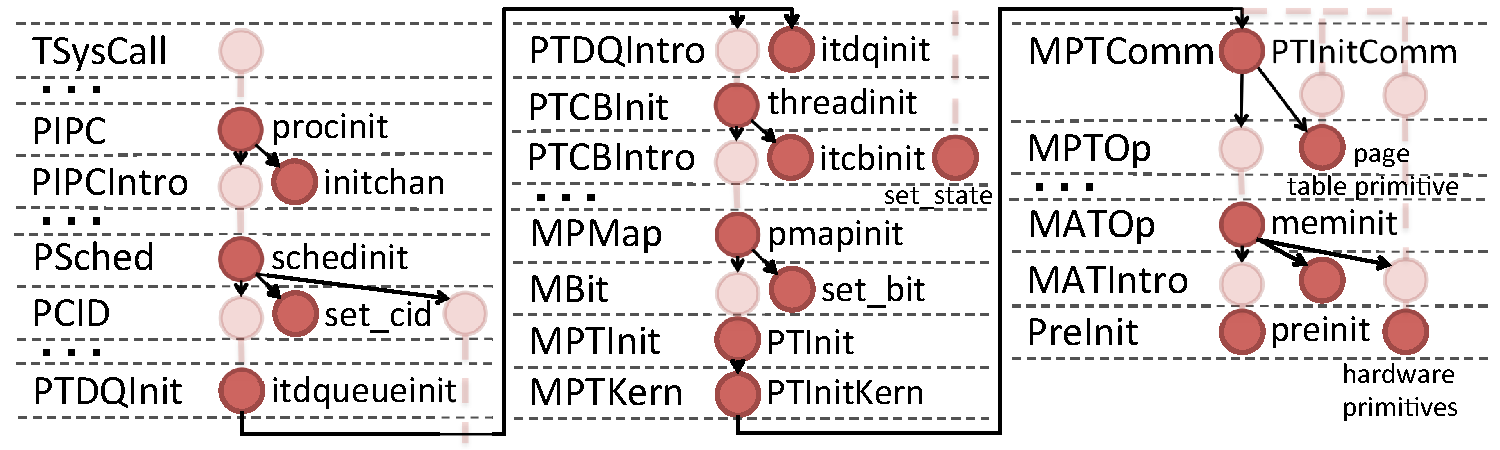
\includegraphics[scale=0.3]{figs/initialization}
\caption{Call graph of \mCTOSbase{} initializer}
\label{fig:mcertikos-init-call-graph}
\end{figure}

%\vspace*{-8pt}
\paragraph{\mCTOShyper{}}
The \mCTOShyper{} kernel provides core primitives to build
full-fledged user-level hypervisors by supporting one of the two
popular hardware virtualization technologies -- AMD SVM.  The primitives
include the operations for manipulating the virtual machine status,
handling VMEXITs, starting or stopping a virtual machine, {\it etc}.
The details of virtualization, e.g., the virtual machine control block
and the nested page table, are hidden from the guest applications.
The hypervisor functionalities are implemented in nine layers and then
inserted in between process management and interrupt handling layers.
The layered approach allows us to do so while (1) only modeling
virtualization-specific structures when needed; (2) retaining
primitives in the layer interface \textsf{PProc} by systematic lifting; and
(3) adding new primitives (including a new initialization function)
guaranteed not to interfere with existing primitives.

%\vspace*{-8pt}
\paragraph{\mCTOSringz{}}
The \mCTOSringz{} kernel explores a different dimension---instead
of adding intermediate layers, we augmented a few existing layers 
(in \mCTOShyper{}) with support of ring 0 processes.
The main modification is at
\textsf{PProc}, where an additional kind of threads is defined.
However, all the layers between \textsf{PProc} and \textsf{TSysCall} also
need to be extended to expose the functionality as system calls.
Thankfully, since all the new primitives are already described in deep
specifications, lifting them to system calls only requires equality
reasoning in Coq.

%\vspace*{-8pt}
\paragraph{\mCTOSembed{}}
The \mCTOSembed{} kernel cuts features down to a bare minimum: it does
not switch to user mode, hence does not require memory protection and
does not provide system call interfaces.  This requires \emph{removing}
features instead of adding them.  Since the layered structure minimizes
entanglements by eliminating unnecessary dependencies and code coupling,
the removal process was relatively easy and straightforward.
Moreover, removing the top 12 layers requires no additional
specifications for those now top-level primitives---deep specifications
are suitable for both internal reasonings and external descriptions.  Thread and process
management layers now sit directly on top of physical memory
management; virtual memory is never enabled.  The
layers remain largely the same barring the removal of primitives
mentioning page tables.

\section{\mCTOSbase{}}
\label{sec:seq:base}

\begin{comment}
\begin{figure*}
\begin{center}
\begin{scriptsize}
\begin{tabular}{ |l|l||l|p{4.5cm}| }
  \hline
  \multicolumn{2}{|c||}{\textbf{Memory Management}} 
  & \multicolumn{2}{|c|}{\textbf{Thread and Process Management}} \\
  \hline
  \hline    
  \multicolumn{2}{|l||}{\textbf{abstract state}} 
  & \multicolumn{2}{|l|}{\textbf{abstract state}}\\
  \hline
  \verb"AT" & physical page allocation table
  & \verb"kctxp" & kernel context (\verb"kctx") pool\\
  \hline 
  \verb"PFInfo" & save the address and \verb"PC" that page fault occurs
  & \verb"Ltdqp" & low abstract thread queue pool\\
  \hline
  \verb"ptp" & page table (\verb"pt") pool 
  
  & \verb"Htdqp"& high abstract thread queue (\verb"Htdq") pool\\ 
  \hline
   \verb"ipt"& whether \verb"pt"'s invariant  should hold or not
  
  & \verb"uctxp" & user context pool\\
  \hline
\verb"PT" & index of the current \verb"pt"
  & \verb"chanp" & channel pool\\
  \hline
  \verb"pbit" & bit map for free \verb"pt" indexes
  & \verb"Htcbp"& high abstract TCB pool \\
  \hline
  \multicolumn{2}{|l||}{\textbf{primitive}} 
  & \multicolumn{2}{|l|}{\textbf{primitive}}\\
  \hline	
  \verb"setcr3" & set the starting address of the \verb"pt"
  & \verb"kctx_new" & allocate the first free \verb"pt" and \verb"kctx"\\
  \hline
  \verb"meminit" & initialize the allocation table
  & \verb"Henqueue" & append a thread to the \verb"Htdq"\\
  \hline
  \verb"palloc" & allocate a page 
  & \verb"thread_kill" & kill and free a thread\\
  \hline
  \verb"pt_insrt" & insert a page map into a given \verb"pt" 
  & \verb"thread_sleep" & sleep, schedule to the 1st ready thread\\
  \hline
  \verb"pt_resv" & allocate a page for a given linear addr 
  & \verb"kctx_switch" & switch \verb"kctx" between threads\\
  \hline 
  \verb"PTInit" & init kernel's \verb"pt" and enable paging 
  & \multirow{2}{*}{\texttt{resv\_chan}} & 
  receive msg from the channel, wake\\
  \cline{1-2}
  \verb"pt_new" & allocate the first free \verb"pt" & & up the first sleeping thread
    \\	  
  \hline
  \hline
  \multicolumn{2}{|c||}{\textbf{Virtualization}}
  &\multicolumn{2}{|c|}{\textbf{Trap Handler}} \\
  \hline
  \hline    
  \multicolumn{2}{|l||}{\textbf{abstract state}} 
  & \multicolumn{2}{|l|}{\textbf{primitive}} \\
  \hline
  \verb"npt" & nested page table for guest
  & \verb"trap_arg" & get arguments of system calls\\
  \hline
  \verb"hctx"& host context
  & \verb"hpagefault" & page fault handler\\ 
  \hline
  \verb"vmcb" & virtual machine (\verb"VM") control control block
  & \verb"sys_yield" & system calls for yielding\\
  \hline
  \verb"xvmst" & registers not saved in \verb"vmcb" 
  & \verb"sys_wait_chan" & system calls to sleep on a channel\\
  \hline
  \multicolumn{2}{|l||}{\textbf{primitive}} 
  & \verb"sys_run_vm" & system calls to run \verb"VM"\\
  \hline	
  \verb"npt_insrt" & insert into the nested page table
  & \verb"sys_proc_create" & system calls to create a process\\
  \hline
  \verb"switch2guest" &  switch to guest mode 
  & \verb"sys_getexitinfo" 
  & get the information about \verb"VM" exit\\
  \hline
  \verb"set_vmcb" & set value in virtual machine control block
  & \verb"sys_injectevent" & inject interrupt and exception to \verb"VM"\\
  \hline 
  \verb"run_vm" & save host context, restore \verb"vmcb", start \verb"VM" 
  & \verb"kernel_init" & initialization function of the kernel\\  
  \hline  

\end{tabular}
\end{scriptsize}
\caption{Key abstract states and primitives for \mCTOSbase{} and \mCTOShyper{}}
\label{table:layers}
\end{center}
\vspace*{-14pt}
\end{figure*}
\end{comment}

The \mCTOSbase{} kernel is divided into six main parts.  From the
bottom layer which corresponds to the physical machine to the top
layer providing system calls, those are the pre-initialization module
(1 layer, Section~\ref{sec:base:preinit},
Fig.~\ref{fig:base:pmm:layers}), physical memory management (3 layers,
Section~\ref{sec:base:pmm}, Fig.~\ref{fig:base:pmm:layers}), virtual
memory management (7 layers, Section~\ref{sec:base:vmm},
Fig.~\ref{fig:base:vmm:layers}), thread management (10 layers,
Section~\ref{sec:base:tm}, Fig.~\ref{fig:base:tm:layers}), process
management (4 layers, Section~\ref{sec:base:pm},
Fig.~\ref{fig:base:pm:layers}), and the trap handler (3 layers,
Section~\ref{sec:base:trap}, Fig.~\ref{fig:base:trap:layers}).  In
this section, we briefly go through each module by describing its
layers from bottom to top.  A detailed description can be found in the
extended TR.

\vspace*{-10pt}
\paragraph{How to read figures describing modules}
In each figure describing a module, each rounded corner box is a layer
with the name in bold. Underneath the name is the list of abstract
states separated by commas. Primitives are enclosed in boxes
touching the bottom edge of the layer; green filling indicates
initialization primitives. Boxes filled with purple represent
a collection of primitives.

Lines with a dot on one end mark refinement relations: the box on the
flat end refines the primitive on the dotted end. On the flat end, the
box can be either a primitive, in the case of \emph{pass-through}
primitives which are implemented in layers further down in the stack,
or a function implementation (an actual piece of code) represented by
a small blue box touching the top of the layer in which it is
implemented.  A function may have outgoing arrows point to primitives
it calls as illustrated in Fig.\ \ref{fig:refine}c; those without
outgoing arrows correspond to Fig.\ \ref{fig:refine}b.

\subsection{Pre-initialization}
\label{sec:base:preinit}

The pre-initialization module is the only trusted component
(assumed to be correct without proofs) in \mCTOSbase{}.
It models the behavior of the underlying machine,
codifying hardware vendors' manuals into mathematical definitions.
Being the bottom layer of \mCTOSbase{},
it is shown at the bottom of Fig.\ \ref{fig:base:pmm:layers} outside the red dashed box.

The abstract states of the pre-initialization module consist of
\verb"MM", \verb"CR3", \verb"PFInfo", and four logical flags.  The
state \verb"MM" is the physical memory map storing the starting
address, end address, and type of each memory piece (see
Fig.\ \ref{fig:abs-pmmap}).  The state \verb"CR3", as its name
suggests, abstracts the CR3 control register, and the state
\verb"FPInfo" abstracts the CR2 control register containing Page Fault
Linear Address (PFLA) as well as the address of the instruction that caused
the page fault.  Finally the four boolean flags \verb"init",
\verb"pe", \verb"ikern", and \verb"ihost" mark whether \verb"preinit"
has been called or not, paging is enabled or not (the PE bit of the
CR0 control register), and the processor is currently in host or guest mode,
or in kernel or user mode.

The main primitive defined in this layer is the initialization function \verb"preinit",
which initializes the abstract state \verb"MM", necessary drivers (tsc, ide, console, {\it etc}),
and interrupts (timer, keyboard, serial, {\it etc}).

\subsection{Physical memory management}
\label{sec:base:pmm} 

{
\setlength{\belowcaptionskip}{-10pt}
\begin{figure}
\begin{center}
\includegraphics[scale=0.31]{figs/pmm_layer}	
\caption{Layers of physical memory management}
\label{fig:base:pmm:layers}
\end{center}
\vspace*{-14pt}
\end{figure}
}

The physical memory management of \mCTOSbase{}
implements the page allocator over 3 layers in the red dashed box in
Fig.\ \ref{fig:base:pmm:layers}.
\ignore{
The module first
defines a getter-setter layer \verb"MATIntro", followed by an
abs-kernel-fun layer \verb"MATOp" where a new initializer is defined,
and then another abs-kernel-fun layer \verb"MAT" which provides the
physical page allocator.
}
The module introduces two new abstract states: \verb"nps", the number
of physical pages, as well as \verb"AT", the page allocation table
indicating whether a memory page is free or not.  The states \verb"AT"
and \verb"nps" are initialized using in \verb"meminit" using the information
in \verb"MM". The module also exports two primitives
\verb"palloc" and \verb"pfree", allocating and freeing memory pages,
respectively.

\ignore{
To verify the implementations of \verb"palloc" and \verb"pfree",
we prove the following invariant at layer \verb"MATOp".
\begin{invariant}
\label{inv:atable}
After the initialization (\verb"init" = \verb"true"),
(1) $2^{18} \le \verb"nps" < 2^{20}$, (2) physical page in low memory part has type \verb"PG_KERNEL", and
(3) physical page in high memory part has type \verb"PG_KERNEL" or \verb"PG_NORMAL".
\end{invariant}

\begin{figure}[ht]\scriptsize
$$
\begin{array}{l|l}
\begin{array}{l}
\verb"typedef enum {"\\
\verb"  PG_RESERVED,"\\
\verb"  PG_KERNEL,"\\
\verb"  PG_NORMAL"\\
\verb"} pg_type;"\\
\\
\verb"struct pginfo {"\\
\verb"  pg_type	t;"\\
\verb"  int	used;"\\
\verb"};"\\
\\
\verb"struct pginfo AT[1<<20];"
\end{array}
&
\begin{array}{l}
\verb+Inductive pg_type :=+\\
\verb+| PG_RESERVED+\\  
\verb+| PG_KERNEL+\\  
\verb+| PG_NORMAL.+\\
\\
\verb+Inductive pginfo :=+\\
\verb+| ATValid (t: pg_type)+\\
\verb+          (used: bool)+\\ 
\verb+| ATUndef.+\\
\\
\verb+Definition AT :=+\\
\verb+      ZMap.t pginfo.+\\
\end{array}
\\\vspace*{-14pt}
\end{array}
$$ 
\caption{Concrete vs. abstract page allocation table}
\label{fig:abs:atable}
\vspace*{-14pt}
\end{figure}

}


\subsection{Virtual memory management}
\label{sec:base:vmm} 

\begin{figure}
\begin{center}
\includegraphics[scale=0.31]{figs/vmm_layer}	
\caption{Layers of virtual memory management}
\label{fig:base:vmm:layers}
\end{center}
\vspace*{-14pt}
\end{figure}

\ignore{
We still focus on memory in the next module, however, we turn our
attention to user programs' needs.  
}
As shown in
Fig.\ \ref{fig:base:vmm:layers}, the virtual memory management of
\mCTOSbase{} consists of 7 layers: getter-setter layer \verb"MPTIntro"
defines two new abstract states, the page map pool \verb"pmp" (which
consists of 64 page tables) and the page map index \verb"pmi" (which
points the current page table); abs-kernel-fun layer \verb"MPTOp"
introduces primitives on page maps including \verb"pt_insrt" and
\verb"pt_read"; the following three abs-kernel-fun layers
\verb"MPTComm", \verb"MPTKern", and \verb"MPTInit" build up the
initialization function \verb"PTInit"; getter-setter layer \verb"MBit"
creates bitmap for page map availability; and, finally,
abs-kernel-fun layer \verb"MPMap" wraps up page map allocation and
release.

Starting from the \verb"MPTIntro" layer, we define the semantics of
address translation (and load/store primitives)
using \verb"pmp" and \verb"pmi" instead of the physical two-level page
table and the \verb"CR3" register.  The contextual refinement relation
between these two kinds of address translations guarantees that the
value in the \verb"CR3" register is always a valid starting address of
a well-formed page table.

\ignore{
\begin{figure}[ht]\scriptsize
$$
\begin{array}{l|l}
\begin{array}{l}
\verb"#define PDES    1024"\\	
\verb"#define PTES    1024"\\
\verb"#define PTEP    0x001"\\
\verb"#define PTEW    0x002"\\
\verb"#define PTEU    0x004"\\
\\
\verb"struct pmap {"\\
\verb"  uint32_t pd[PDES];"\\
\verb"  uint32_t pt[PDES][PTES];"\\
\verb"};"\\
\\
\verb"struct pmap pmp[64];"
\end{array}
&
\begin{array}{l}
\verb+Inductive PTPerm :=+\\
\verb+| PTEP | PTEW | PTEU.+\\
\verb+Inductive PTE:=+\\
\verb+| PTEV (v: block)+\\
\verb+       (p: PTPerm)+\\
\verb+| PTEUnPresent+\\
\verb+| PTEUndef.+\\
\verb+Definition PT :=+\\
\verb+      ZMap.t PTE.+\\
\verb+Inductive PDE :=+\\
\verb+| PDEV (pt: PT)+\\
\verb+| PDEUndef.+\\
\verb+Definition pmap :=+\\
\verb+      ZMap.t PDE.+\\
\verb+Definition pmp :=+\\
\verb+      ZMap.t pmap.+
\end{array}
\\\vspace*{-14pt}
\end{array}
$$ 
\caption{Concrete vs. abstract page table}
\label{fig:abs:ptable}
\end{figure}

Since \verb"PTInit"  enables paging after initializing \verb"pmp", the addressing mode changes inside the function execution. Therefore, verification of the initialization function need to enforce that:
\begin{invariant}
\label{inv:pagemap}
When paging is enabled (\verb"pe" = \verb"true"),
(1) the low memory part of all page maps in \verb"pmp" must be identity maps, and
(2) if in the kernel mode (\verb"kern" = \verb"true"), the current page table (\verb"pmp[pmi]") must be an identity map.
\end{invariant}
}


\subsection{Thread management}
\label{sec:base:tm} 

{
\setlength{\belowcaptionskip}{-10pt}
\begin{figure}
\begin{center}
\includegraphics[scale=0.31]{figs/tm_layer}	
\caption{Layers of thread management}
\label{fig:base:tm:layers}
\end{center}
\vspace*{-14pt}
\end{figure}
}

\ignore{
\begin{figure}[ht]\scriptsize
$$
\begin{array}{l|l}
\begin{array}{l}
\verb+Record thread := {+\\
\verb+  id: Z;+\\ 
\verb+  kernel_context: kctx;+\\
\verb+  TCB: tcb;+\\
\verb+  sleep_queue: tdq+\\
\verb+}+
\end{array}
&
\begin{array}{l}
\verb+Record process := {+\\
\verb+  td: thread;+\\
\verb+  pagemap: pmap;+\\
\verb+  user_context: uctx;+\\
\verb+  channel: chan+\\
\verb+}+
\end{array}
\\\vspace*{-14pt}
\end{array}
$$ 
\caption{Abstract thread and process}
\label{fig:abs:threadproc}
\end{figure}
}


The thread management module consists of 10 layers and is
shown in Fig.~\ref{fig:base:tm:layers}.  The layers \verb"PKCtx",
\verb"PTCBIntro", and \verb"PTDQIntro" are getter-setter layers
defining the kernel context pool \verb"kctxp", the intermediate
abstract thread control block (TCB) pool \verb"itcbp", and the
intermediate thread queue pool \verb"itdqp", respectively, while
\verb"PKCtxOp", \verb"PTCBInit", and \verb"PTDQInit" are
abs-kernel-fun layers introducing operations over these abstract
states. The top four layers then finalize the abstraction into the
thread pool \verb"threadp", the ready queue \verb"rdq", and the
current thread id \verb"cid", and provide the standard thread
primitives such as \verb"thread_spawn" and \verb"thread_yield".

{
\setlength{\floatsep}{-10pt}
\setlength{\belowcaptionskip}{-10pt}
\vspace*{-10pt}
\begin{figure}[ht]\tiny
$$
\begin{array}{l|l}
\begin{array}{l}
\verb+struct tcb *+\\
\verb+dequeue(struct tdq * queue){+\\
\verb+  struct tcb * head, next;+\\
\verb+  struct tcb * pid = null;+\\
\verb+  if(queue == null)+\\
\verb+    return pid;+\\
\verb+  else {+\\
\verb+    head = queue -> head;+\\
\verb+    if (head == null)+\\
\verb+      return pid;+\\
\verb+    else {+\\
\verb+      pid = head;+\\
\verb+      next = head -> next;+\\
\verb+      if(next == null) {+\\
\verb+        queue -> head = null;+\\
\verb+        queue -> tail = null;+\\
\verb+      } else {+\\
\verb+        next -> prev = null;+\\
\verb+        queue -> head = next;+\\
\verb+      }+\\
\verb+    }+\\
\verb+  }+\\
\verb+  return pid;+\\
\verb+}+
\end{array}
&
\begin{array}{l}
\verb+Function dequeue (d:abs) (i:Z) :=+\\
\verb+match d.itdqp i with+\\
\verb+|TDQV h t =>+\\
\verb+ if zeq h null then+\\
\verb+  Some (d, null)+\\
\verb+ else+\\
\verb+  match d.itcbp h with+\\
\verb+  |TCBV _ n =>+\\
\verb+   if zeq n null then+\\
\verb+   let tdq':=(TDQV null null) in+\\
\verb+    Some (set_itdq d i tdq', h)+\\
\verb+   else+\\ 
\verb+    match d.itcbp n with+\\
\verb+    |TCBV s' _ n' =>+\\
\verb+    let tdq':=(TDQV n t) in+\\
\verb+    let d':=set_itdq d i tdq' in+\\
\verb+    let tcb':=(TCBV s' null n') in+\\
\verb+      Some (set_itcb d' n tcb', h)+\\
\verb+    |_ => None+\\
\verb+    end+\\
\verb+  |_ => None+\\
\verb+  end+\\
\verb+|_ => None+\\
\verb+end+
\end{array}
\vspace*{-14pt}
\end{array}
$$ 
\caption{Concrete vs. intermediate dequeue primitive}
\label{fig:abs:dequeue}
\end{figure}
}

{
\setlength{\floatsep}{-10pt}
\setlength{\abovecaptionskip}{3pt}
\setlength{\belowcaptionskip}{-10pt}
\begin{figure}[ht]\scriptsize
\begin{verbatim}
    Function dequeue (d:abs) (i:Z) :=
      match d.tdqp i with
        | h :: q => Some (set_tdq d i q, h)
        | nil => None 
      end 
\end{verbatim}
\vspace*{-14pt}
\caption{Abstract dequeue primitive}
\label{fig:abs:Hdequeue}
\end{figure}
}

{
\setlength{\floatsep}{-10pt}
\setlength{\belowcaptionskip}{-5pt}
\begin{figure}[ht]\scriptsize
$$
\begin{array}{l|l}
\begin{array}{l}
\verb+Inductive itcb :=+\\
\verb+| TCBUndef+\\
\verb+| TCBV (tds: td_state)+\\
\verb+       (prev next: Z)+\\
\\
\verb+Definition itcbp:=+\\
\verb+      ZMap.t itcb+
\end{array}
&
\begin{array}{l}
\verb+Inductive itdq :=+\\
\verb+| TDQUndef+\\
\verb+| TDQV (head tail: Z)+\\
\\
\verb+Definition itdqp:=+\\
\verb+      ZMap.t itdq+
\end{array}
\vspace*{-14pt}
\end{array}
$$ 
\caption{Intermediate abstract TCB and thread queue}
\label{fig:abs:ltdq}
\end{figure}
}

In Fig.~\ref{fig:spec:tdq} of Sec.~\ref{sec:spec:layerdefine}, we
presented the concrete implementations of the thread control blocks
and thread queues (using doubly linked lists) as well as the abstract
view of these data structures using Coq lists.  The abstraction 
makes reasoning easier and is used to describe the behaviors of
functions that operate on these data structures.

As an example, the C implementation of the operation \verb"dequeue" is shown
in the left panel of Fig.\ \ref{fig:abs:dequeue} and the corresponding
abstract specification is shown in Fig.\ \ref{fig:abs:Hdequeue}.
Unfortunately, the drastic difference between the two renders
the verification extremely complicated.

To the rescue, again, is the layering design.  The fact that the two
layers are too far apart (to be easily verifiable) calls for more
layers in between.  Recall that layered specification and verification
aim at specifying and verifying each implementation at the right
abstraction level.  The Coq list is apparently too high an abstraction
for the doubly linked list and we should find a middle ground between
them.  One major gap between the two is that in a doubly linked list,
a node {\em contains} references to the next and the previous nodes,
while in a Coq list, it is the \verb"cons" cell that holds the link to
the current and the next nodes.

This is why we introduce the intermediate abstract TCB and thread
queue in the bottom 6 layers in this module.  The definitions of the
intermediate data structures are listed in Fig.\ \ref{fig:abs:ltdq} and
the dequeue function is shown in the right panel of
Fig.\ \ref{fig:abs:dequeue}.  Since we store the previous and next
nodes as numbers in \verb"itcb", we are able to mimic the C code
closely, resulting in a much simpler proof.

Based on these intermediate layers, we then introduce the
\verb"PAbQueue" layer, which contains the TCB and queue definitions in
Fig.\ \ref{fig:spec:tdq} and the dequeue function in
Fig.\ \ref{fig:abs:Hdequeue}. This layer is then used to define
primitives on threads.  It still takes some effort to prove the
refinement relation but it is more manageable as they are both Coq
functions. 

\ignore{
\begin{invariant}
\label{inv:tdqueue}
(1) Every thread with the state \verb"TD_READY" is in the ready queue;
(2) Every thread with the state \verb"TD_SLEEP" is in one and only one sleeping queue;
(3) All other threads are neither in the ready queue nor in any of the sleeping queues.
\end{invariant}
}

\ignore{
As shown in Fig.~\ref{fig:abs:threadproc} (left), an abstract thread \verb"thread" consists of the thread id, kernel context, TCB and a sleeping queue.
}

\begin{comment}
(In the figure, abstract states and primitives are abbreviated as \verb"mm.abs" and \verb"mm.prim", marked as purple.)
\end{comment}

\subsection{Process management}
\label{sec:base:pm} 


{
\setlength{\belowcaptionskip}{-10pt}
\begin{figure}
\begin{center}
\includegraphics[scale=0.31]{figs/pm_layer}	
\caption{Layers of process management}
\label{fig:base:pm:layers}
\end{center}
\vspace*{-14pt}
\end{figure}
}
 
Fig.\ref{fig:base:pm:layers} shows the 4 layers of the process
management module.  The layers \verb"PIPCIntro", and
\verb"PIPC" are the getter-setter layer and abs-kernel-fun layer for
inter-process communication (IPC) channel pool \verb"chanp".  The
layer \verb"PUCtx" is the getter-setter layer for user context pool
\verb"uctxp", while the layer \verb"PProc" introduces
the abstract process pool \verb"procp" and primitives to manage
processes.

\ignore{
As shown in Fig.~\ref{fig:abs:threadproc} (right),
an abstract \verb"process" consists of a kernel thread, a page map,
a user context, and an IPC channel.
}

\subsection{Trap handler}
\label{sec:base:trap}

\begin{figure}[ht]
\begin{center}
\includegraphics[scale=0.3]{figs/trap_layer_base}	
\caption{Layers of trap handler}
\label{fig:base:trap:layers}
\end{center}
\vspace*{-14pt}
\end{figure}

{
\setlength{\belowcaptionskip}{-10pt}
\begin{figure}
\begin{center}
\includegraphics[scale=0.3]{figs/pagefault}	
\caption{Call graph of page fault handler}
\label{fig:base:trap:pagefault}
\end{center}
\vspace*{-14pt}
\end{figure}
}

The trap handler module of \mCTOSbase{} consists of 3 abs-kernel-fun
layers, shown in Fig\ ~\ref{fig:base:trap:layers}.  It specifies the
trap handler module in the standard operating system.  The
\verb"TTrapArg" layer introduces primitives to manage the system call
arguments and return values, while the \verb"TTrap" layer implements
the necessary handlers for system calls and exceptions.  Finally, the
\verb"TSysCall" layer specifies the semantics of system calls from the
user point of view, following the x86 system call convention.

The behavior that saves and restores the trap frame (user context)
structure is modeled with the primitives \verb"proc_exit" and
\verb"proc_start".  The verified assembly implementation only saves
and restores the second half of the user context as the first half is
saved and restored by the hardware.  For the exception handler, we
implement the standard page fault handler which dynamically allocates
the user memory in the page table.  Fig.~\ref{fig:base:trap:pagefault}
shows the call graph of our page fault handler. 
\ignore{
Here, red
points are primitives at different layers, edges represent
invocations, and the primitives are called from left to right in the
order of the edges. 
}
We can see that the
implementation of the page fault handler involves 18 primitives across
12 layers.  On the other hand, the verification of the handler is
fairly simple as it is specified using abstract specifications of the
functions it directly calls on a layer with a very high level of
abstraction (\verb"TTrap").


\ignore{
\subsectskip
\subsection{User-level program}
\label{sec:base:user}
\asubsectskip

Thanks to the contextual refinement relation that we have built between the system call primitives and the underlying kernel implementations, we can reason about the user-level program with the specification of system calls and linked the proof with the one of \mCTOSbase{}.

For example, suppose we have verified that a user process $U$ linked with the system call specifications satisfy the specification $S$, which is
$$
\sem{\rm\mCTOSbase{}}{U}\Refrel{}\sem{}{S}
$$

By the final theorem of \mCTOSbase{} we have proved, 
$$
\forall P,\;\sem{\rm{}x86}{K\join{}P}\Refrel{}\sem{\rm\mCTOS}{P}
$$
, and instantiate $P$ with $U$, we can get the theorem that
$$
\sem{\rm{}x86}{U\join{}K}\Refrel{}\sem{}{S}
$$
, meaning that the user program $U$ linked with the kernel implementation $K$ and running on a x86 bare machine still satisfy the specification $S$.

%% To be moved to POPL: OSDI do not care about C vs. Asm
%%However, one limitation is that, we could not link a certified compiler using flat memory model with \mCTOSbase{}. It means that we can only verify the user-level program at assembly level instead of at C level.

\ronghui{
\begin{itemize}
\item Maybe we can find some interesting user programs
%% \item We can also put the limitation to the section 7. --> moved to POPL
\item where to put the final theorem
\end{itemize}
}
}
